%!Tex Root = ../Main.tex
% ./Motivation.tex
% ./Einführung.tex
% ./Implementierung.tex
% ./Ergebnisse_und_Ausblick.tex
\documentclass{report}
\usepackage[showframe, margin=1.5cm]{geometry}
\usepackage[ngerman]{babel}
\usepackage{lipsum}
\usepackage[parfill, ]{parskip}
\setlength{\parskip}{0.4cm} % space between paragraphs
\usepackage{setspace}
\usepackage{graphicx}
\usepackage[colorlinks=true, allcolors=PrimaryColor]{hyperref} %hidelinks

% colorbox stuff
\usepackage{tcolorbox}
\usepackage{tikz}
\tcbuselibrary{skins}
\tcbuselibrary{breakable}
\usetikzlibrary{patterns}
\usetikzlibrary{shadings}
\tcbuselibrary{theorems}
\tcbuselibrary{listings}
% https://tex.stackexchange.com/questions/550052/command-parboxrestore-has-changed
\tcbuselibrary{minted}
\tcbset{listing engine=minted}
% \tcbuselibrary{raster}

\usepackage{cleveref}

\usepackage{csquotes}
\usepackage[style=authortitle]{biblatex}
\addbibresource{./My Library/My Library.bib}
\usepackage{pdfpages}
\usepackage{booktabs} % for table rules
\usepackage{tabulary}
% \usepackage{tabularx}
\usepackage{array}
\usepackage{multirow}
\usepackage{amssymb}

% https://tex.stackexchange.com/questions/9425/how-to-fix-footnote-position-at-the-bottom-of-the-page
\usepackage[bottom, flushmargin]{footmisc}

% https://tex.stackexchange.com/a/32212
\interfootnotelinepenalty=10000

% https://tex.stackexchange.com/questions/8625/force-figure-placement-in-text
\usepackage{float}

\usepackage{xcolor}
\definecolor{PrimaryColor}{HTML}{4D2875}
\definecolor{SecondaryColor}{HTML}{DBD3E3}


\newcommand{\smalltt}[1]{{\small\texttt{#1}}}

% bold with color
\newcommand\colorbold[1]{\textcolor{PrimaryColor}{\textbf{#1}}}

% https://tex.stackexchange.com/questions/153167/how-to-set-page-number-at-right-footer
% footer
\usepackage{fancyhdr}
\pagestyle{fancy}
\fancyhf{}
\fancyfootoffset{1cm}
\rfoot[]{\thepage}

\fancypagestyle{plain}{%
  % on first chapter pages no rule
    \renewcommand{\headrulewidth}{0mm}%
    \fancyhf{}%
    \rfoot[]{\thepage}
}

% header
\fancyheadoffset{1cm}
\lhead{\nouppercase{\leftmark}}
\rhead{\nouppercase{\rightmark}}

% https://tex.stackexchange.com/questions/108684/spacing-before-and-after-section-titles
% spacing after section
\usepackage{titlesec}

% \titlespacing*{\section}
\titlespacing*{\section}{0cm}{*4}{*4}
\titlespacing*{\subsection}{0cm}{*3}{*3}
\titlespacing*{\subsubsection}{0cm}{*2}{*2}

% https://tex.stackexchange.com/questions/139366/chapter-header-with-super-huge-numbers
\usepackage{fix-cm}
\newcommand{\hsp}{\hspace{0pt}}
\titleformat{\chapter}[hang]{\bfseries}{\fontsize{100}{0}\selectfont \textcolor{PrimaryColor}\thechapter\hsp}{0.5cm}{\Huge}[]

% https://tex.stackexchange.com/a/40001
\titlespacing*{\chapter}{0cm}{*0}{*4}

% https://golatex.de/viewtopic.php?t=18830
\defbibenvironment{bibliography}
  {\itemize}
  {\enditemize}
  {\item}

% https://tex.stackexchange.com/questions/358292/creating-a-subcounter-to-a-counter-i-created
\usepackage{chngcntr}

% https://tex.stackexchange.com/questions/18870/defining-an-new-itemize-like-environment-where-itemfoo-passes-foo-to-a-macro
\usepackage{ifmtarg}

% https://tex.stackexchange.com/questions/8351/what-do-makeatletter-and-makeatother-do
\makeatletter

% ignorespace: https://runebook.dev/de/docs/latex/_005cignorespaces-_0026-_005cignorespacesafterend
% enspace: https://math-linux.com/latex-26/faq/latex-faq/article/latex-horizontal-space-qquad-hspace-thinspace-enspace
\newcommand{\coloritem[1]}[]{%
\@ifmtarg{#1}{\item[\textcolor{PrimaryColor}{\textbullet}]}%
{\item[\textcolor{PrimaryColor}{\textbullet}] \colorbold{\textbf{#1:}}}\enspace\ignorespaces}

\makeatother

% https://stackoverflow.com/questions/1061112/eliminate-space-before-beginitemize
\usepackage{enumitem}

% https://tex.stackexchange.com/a/263470
\usepackage{microtype}

% https://tex.stackexchange.com/questions/165178/nameref-hyperref-evaluating-counter-instead-of-section-name
\usepackage{nameref}
\GetTitleStringSetup{expand}

% https://stackoverflow.com/questions/1078370/subfigs-of-a-figure-on-multiple-pages
\usepackage{subfig}

% https://tex.stackexchange.com/questions/130795/how-can-i-number-sections-below-subsection-in-latex
\setcounter{secnumdepth}{5}

% https://tex.stackexchange.com/questions/32160/new-line-after-paragraph
\newcommand{\newlineparagraph}[1]{\paragraph{#1}\mbox{}\\\vspace{-0.5cm}}
 % ./content/Packete_und_Deklarationen.tex

\includeonly{
  ./content/Motivation,
  ./content/Einführung,
  ./content/Implementierung,
  ./content/Ergebnisse_und_Ausblick,
  ./content/Appendix
}


\begin{document}
  \sloppy

  \newtcolorbox{titlebox}[1]{skin=enhanced, arc=0mm, boxrule=0mm,
      title style={preaction={fill=PrimaryColor}, pattern=fivepointed stars, pattern color=white, opacity=0.1},
      interior style={preaction={fill=SecondaryColor}, pattern=fivepointed stars, pattern  color=white, opacity=0.3},
      frame style={color=white},
      % segmentation style={black,solid,opacity=0.2,line width=1pt}
      title={#1}
    }

  %!Tex Root = ../Main.tex
% ./Packete_und_Deklarationen.tex

\begin{titlepage}
  \vspace{1cm}
  \center
  \textsc{\LARGE Albert Ludwigs Universität Freiburg}\\[0.5cm]
  \textsc{\Large Technische Fakultät}\\[2.0cm]

  \vspace{1cm}

  \begin{titlebox}{\center \huge \bfseries PicoC-Compiler}
    \center
    % \\
    % \tcblower
    {\bfseries \center \LARGE \setstretch{1.1} Übersetzung einer Untermenge von C in den Befehlssatz der RETI-CPU\par}
  \end{titlebox}
    \textsc{\large Bachelorarbeit}\\
    \rule{\linewidth}{0.1mm}\\[0.5cm]

  {\large \emph{Abgabedatum:} 28\textsuperscript{th} April 2022}\\[2.5cm]

  \begin{minipage}{0.45\textwidth}
    \begin{flushleft} \large
      \emph{Author:}\\
      Jürgen Mattheis\\
      \hspace{1cm}\\
      \hspace{1cm}\\
      \hspace{1cm}\\
      \hspace{1cm}
    \end{flushleft}
  \end{minipage}
  ~
  \begin{minipage}{0.45\textwidth}
    \begin{flushright} \large
      \emph{Gutachter:}\\
      Prof. Dr. Scholl\\[0.64cm]
      \emph{Betreung:}\\
      M.Sc. Seufert\\
    \end{flushright}
  \end{minipage}

  \vspace{8.cm}
  \rule{11cm}{0.1mm}\\[0.25cm]
  \large{Eine Bachelorarbeit am Lehrstuhl für}\\
  \large{Betriebssysteme}
\end{titlepage}
                 % ./content/Titlepage.tex
  \newgeometry{margin=2.5cm}
  \setlength{\footskip}{30pt}                 % move pagenumber up and down
  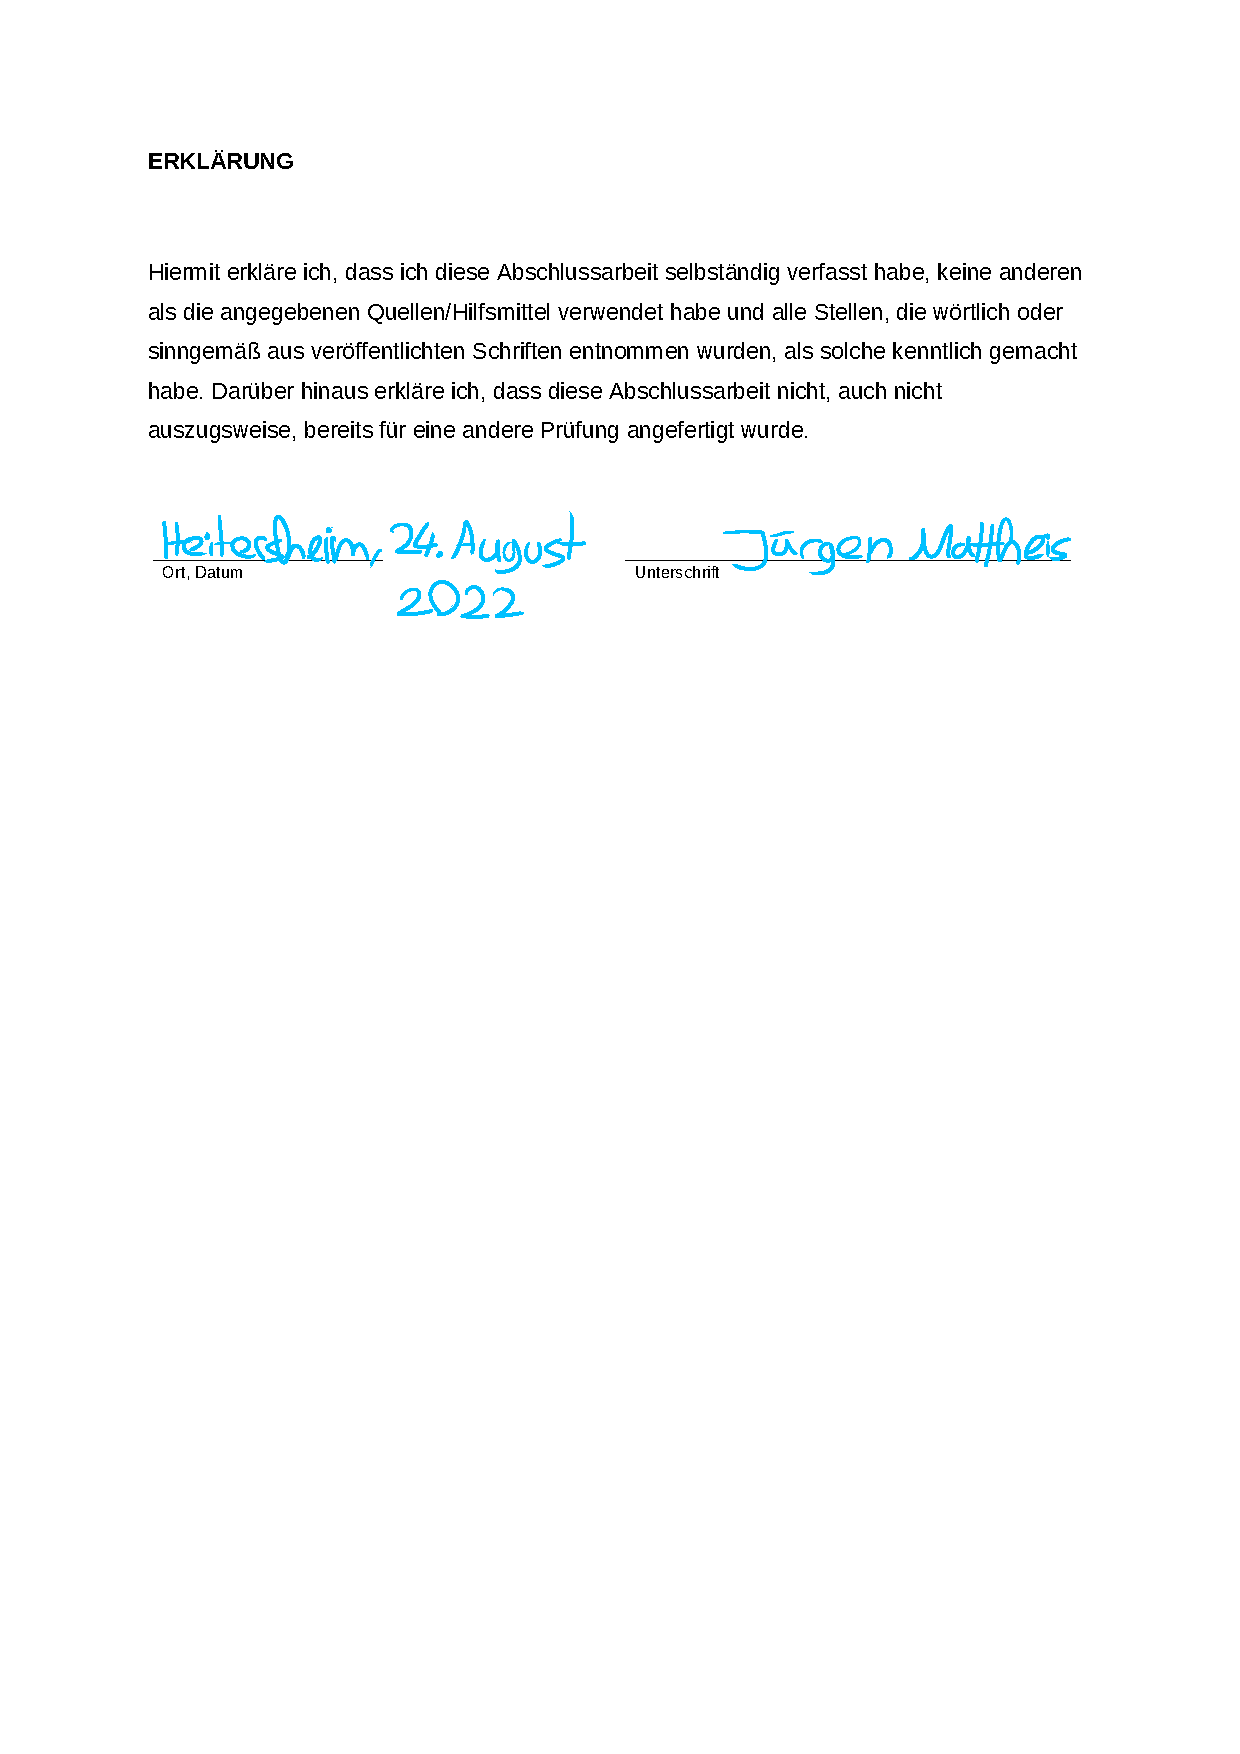
\includepdf[pages=-]{./ErklrungfrdieAbschlussarbeit_unterschrieben.pdf}

  \tableofcontents
  \listoffigures
  \listoftables
  % https://tex.stackexchange.com/questions/538528/tcolorbox-newtcbtheorem-index-with-tcolorbox
  \tcblistof[\chapter*]{theorem_list}{Definitionen}

  \newtcbtheorem[list inside={theorem_list},crefname={definition}{definitions}, number within=chapter]{Definition}{Definition}%
  {enhanced, arc=0mm,top=3mm,bottom=3mm, boxrule=0mm, borderline south={1mm}{0pt}{PrimaryColor}, title style={color=PrimaryColor},
  interior style={opacity=0.2, fill=PrimaryColor},
  frame style={color=white}, fonttitle=\bfseries, fontupper=\itshape,
  before upper=\setlength{\parskip}{1em}
  }{def}

  \newtcolorbox{Special_Paragraph}{enhanced, breakable, arc=0mm, left=3mm, right=3mm, boxrule=1mm, borderline vertical={1mm}{0pt}{PrimaryColor},
  interior style={fill=SecondaryColor},
  frame style={color=white},
  % https://tex.stackexchange.com/questions/459870/paragraph-breaks-inside-tcolorbox, maybe also parbox=false
  before upper=\setlength{\parskip}{1em}
  }

  \newtcbinputlisting{\codebox}[2][]{
  listing file={#2},
  enhanced, colframe=PrimaryColor,colback=SecondaryColor, fonttitle=\bfseries, width=0.25\linewidth, arc=0mm, #1, listing only, minted language=C, halign title=center
  }
  % minted language=C,

  \newtcbinputlisting{\treebox}[2][]{
  listing file={#2},
  enhanced, colframe=PrimaryColor, colback=SecondaryColor, fonttitle=\bfseries, width=0.25\linewidth, arc=0mm, #1, listing only, halign title=center
  }

  %!Tex Root = ../Main.tex
% ./Packete_und_Deklarationen.tex
\chapter{Motivation}
\label{ch:motivation}

\section{PicoC und RETI}
\section{Aufgabenstellung}
% erweitern des Compilers aus dem Bachelorprojekt
\section{Eigenheiten der Sprache C}
% Abhängigkeit von Typ von Variable usw.
% Designfehler
% Spiral Rule
% Specifier, die ganzen Begriffe aus calcourse
\section{Richtlinien}
% Email an Scholl
% exakt gleiche Präzidenzregeln
% kein unnötiger Schnickschnack
              % ./content/Motivation.tex
  \include{./content/Einführung}              % ./content/Einführung.tex
  %!Tex Root = ../Main.tex
% ./Packete_und_Deklarationen.tex
% ./Titlepage.tex
% ./Motivation.tex
% ./Einführung.tex
% ./Ergebnisse_und_Ausblick.tex

\chapter{Implementierung}
\label{ch:implementierung}
\section{Architektur}
% Unterscheid zur Architektur aus dem Bachelorprojekt

% Cross Compiler
\begin{figure}
  \centering
  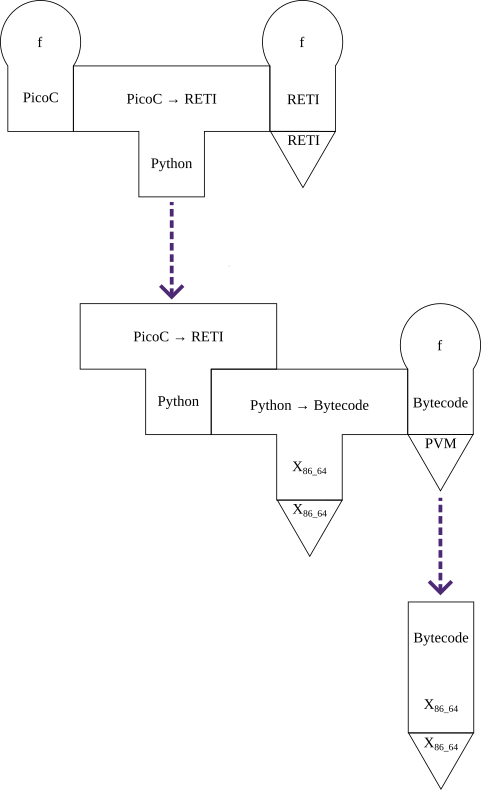
\includegraphics[width=0.5\linewidth]{./figures/summarized_cross_compiler.png}
  \caption{Cross-Compiler Kompiliervorgang ausgeschrieben}
\end{figure}

\begin{figure}
  \centering
  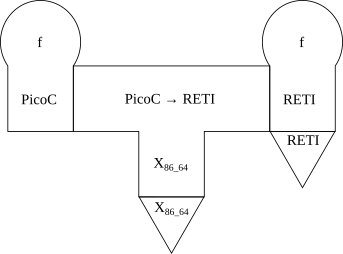
\includegraphics[width=0.33\linewidth]{./figures/compiliervorang_mit_machiene.png}
  \caption{Cross-Compiler Kompiliervorgang Kurzform}
\end{figure}

\begin{figure}
  \centering
  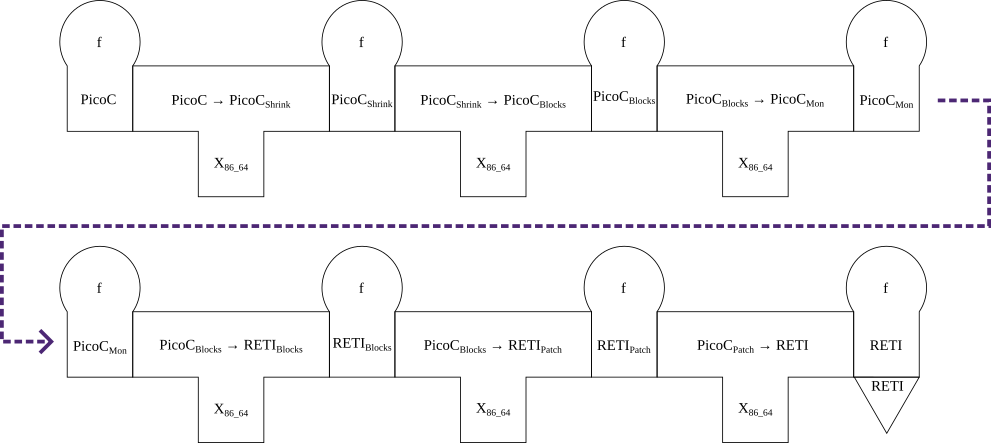
\includegraphics[width=\linewidth]{./figures/passes.png}
  \caption{Architektur mit allen Passes ausgeschrieben}
\end{figure}

\section{Lexikalische Analyse}
\subsection{Verwendung von Lark}
% erwähnen, dass in Lark die Grammatiken L_Lex und L_Parse gemischt sind
% EBNF erwähnen
% (erwähnen, dass finalle Grammatik im Appendix)
\subsection{Basic Parser}
\section{Syntaktische Analyse}
\subsection{Verwendung von Lark}
% Vorteile von Lark
\subsection{Umsetzung von Präzidenz}
Die \colorbold{PicoC Sprache} hat dieselben \colorbold{Präzidenzregeln} implementiert, wie die \colorbold{Sprache C} \footcite{noauthor_c_nodate}. Die \colorbold{Präzidenzregeln} von \colorbold{PicoC} sind in Tabelle~\ref{tab:reference_table} aufgelistet.

\begin{table}[H]
  \center
  \begin{tabulary}{\linewidth}{|C|C|L|L|}
  \toprule
  \colorbold{Präzidenz} &	\colorbold{Operator} & \colorbold{Beschreibung} &	\colorbold{Assoziativität} \\
  \midrule
  1	& \verb|a()|	& Funktionsaufruf & \multirow{2}{=}{Links, dann rechts $\rightarrow$} \\
    & \verb|a[]|	& Indexzugriff & \\
    & \verb|a.b| & Attributzugriff & \\
  \hline
  2	&	\verb|-a| & Unäres Minus & \multirow{2}{=}{Rechts, dann links $\leftarrow$} \\
    & \smalltt{!a $\thicksim$a}	& Logisches NOT und Bitweise NOT & \\
    & \verb|*a &a| & Dereferenz und Referenz, auch Adresse-von & \\
  \hline
  3	& \smalltt{a*b a/b a\%b} &	Multiplikation, Division und Modulo & Links, dann rechts $\rightarrow$ \\
  \cline{1-3}
  4	& \verb|a+b a-b|	& Addition und Subtraktion & \\
  \cline{1-3}
  5	& \verb|a<b a<=b| \verb|a>b a>=b| & Kleiner, Kleiner Gleich, Größer, Größer gleich & \\
  \cline{1-3}
  6 &	\verb|a==b a!=b| & Gleichheit und Ungleichheit & \\
  \cline{1-3}
  7 &	\verb|a&b| & Bitweise UND & \\
  \cline{1-3}
  8 &	\verb|a^b| & Bitweise XOR (exclusive or) & \\
  \cline{1-3}
  9 & \smalltt{a$\mid$b} & Bitweise ODER (inclusive or) & \\
  \cline{1-3}
  10	& \verb|a&&b| &	Logiches UND & \\
  \cline{1-3}
  11	& $a{\mid\mid} b$	& Logisches ODER & \\
  \hline
  12 & \verb|a=b| & Zuweisung & Rechts, dann links $\leftarrow$ \\
  \hline
  13 &	\verb|a,b|& Komma	& Links, dann rechts $\rightarrow$ \\
  \bottomrule
\end{tabulary}
\caption{Präzidenzregeln von PicoC}
\label{tab:reference_table}
\end{table}
% erwähnen von Mehrdeutigkeit und Assoziativität
% finalle Grammatik im Appendix
% Crafting Compilers Quelle benennen
\subsection{Derivation Tree Generierung}
\subsection{Early Parser}
\subsection{Derivation Tree Vereinfachung}
% Visitor erwähnen
\subsection{Abstrakt Syntax Tree Generierung}
\subsubsection{ASTNode}
\subsubsection{PicoC Nodes}
% Tabelle aller PicoC Nodes
% möglichst kurze und leicht verständliche Bezeichner für Nodes
\subsubsection{RETI Nodes}
% Tabelle aller RETI Nodes
% Transformer erwähnen
\section{Code Generierung}
\subsection{Passes}
\subsubsection{PicoC-Shrink Pass}
% dieser Pass wurde wegen
\subsubsection{PicoC-Blocks Pass}
\subsubsection{PicoC-Mon Pass}
\begin{Definition}{Symboltabelle}{symboltabelle}
\end{Definition}
\subsubsection{RETI-Blocks Pass}
\subsubsection{RETI-Patch Pass}
\subsubsection{RETI Pass}
% TODO: zusammenfassendes Bild

\subsection{Umsetzung von Pointern}
\subsubsection{Referenzierung}
\begin{code}
  \centering
  \numberedcodebox[minted language=c]{./code_examples/example_pntr_ref.picoc}
  \caption{PicoC Code für Pointer Referenzierung}
  \label{fig:picoc_code_für_pointer_referenzierung}
\end{code}

\begin{code}
  \centering
  \numberedcodebox[minted language=text]{./code_examples/example_pntr_ref.ast}
  \caption{Abstract Syntax Tree für Pointer Referenzierung}
  \label{fig:abstract_syntax_tree_für_pointer_referenzierung}
\end{code}

\begin{code}
  \centering
  \numberedcodebox[minted language=text]{./code_examples/example_pntr_ref.picoc_mon}
  \caption{PicoC Mon Pass für Pointer Referenzierung}
  \label{fig:picoc_mon_für_pointer_referenzierung}
\end{code}

\begin{code}
  \centering
  \numberedcodebox[minted language=text]{./code_examples/example_pntr_ref.reti_blocks}
  \caption{RETI Blocks Pass für Pointer Referenzierung}
  \label{fig:reti_blocks_für_pointer_referenzierung}
\end{code}
% Initialisierung eines Pointers
\subsubsection{Pointer Dereferenzierung durch Zugriff auf Arrayindex ersetzen}
\begin{code}
  \centering
  \numberedcodebox[minted language=c]{./code_examples/example_pntr_deref.picoc}
  \caption{PicoC Code für Pointer Dereferenzierung}
  \label{fig:picoc_code_für_pointer_dereferenzierung}
\end{code}

\begin{code}
  \centering
  \numberedcodebox[minted language=text]{./code_examples/example_pntr_deref.ast}
  \caption{Abstract Syntax Tree für Pointer Dereferenzierung}
  \label{fig:abstract_syntax_tree_für_pointer_dereferenzierung}
\end{code}

\begin{code}
  \centering
  \numberedcodebox[minted language=text]{./code_examples/example_pntr_deref.picoc_shrink}
  \caption{PicoC Shrink Pass für Pointer Dereferenzierung}
  \label{fig:picoc_shrink_für_pointer_dereferenzierung}
\end{code}

\subsection{Umsetzung von Arrays}
\subsubsection{Initialisierung von Arrays}
% Stack und Globale Statische Daten
\begin{code}
  \centering
  \numberedcodebox[minted language=c]{./code_examples/example_array_init.picoc}
  \caption{PicoC Code für Array Initialisierung}
  \label{fig:picoc_code_für_array_initialisierung}
\end{code}

\begin{code}
  \centering
  \numberedcodebox[minted language=text]{./code_examples/example_array_init.ast}
  \caption{Abstract Syntax Tree für Array Initialisierung}
  \label{fig:abstract_syntax_tree_für_array_initialisierung}
\end{code}

\begin{code}
  \centering
  \numberedcodebox[minted language=text]{./code_examples/example_array_init.picoc_mon}
  \caption{PicoC Mon Pass für Array Initialisierung}
  \label{fig:picoc_mon_für_array_initialisierung}
\end{code}

\begin{code}
  \centering
  \numberedcodebox[minted language=text]{./code_examples/example_array_init.reti_blocks}
  \caption{RETI Blocks Pass für Array Initialisierung}
  \label{fig:reti_blocks_für_array_initialisierung}
\end{code}


% kleines Extra
\subsubsection{Zugriff auf Arrayindex}
Der Zugriff auf einen bestimmten  Index eines Arrays ist wie folgt umgesetzt:

\begin{code}
  \centering
  \numberedcodebox[minted language=c]{./code_examples/example_array_access.picoc}
  \caption{PicoC Code für Zugriff auf Arrayindex}
  \label{fig:picoc_code_für_zugriff_auf_arrayindex}
\end{code}

\begin{code}
  \centering
  \numberedcodebox[minted language=text]{./code_examples/example_array_access.ast}
  \caption{Abstract Syntax Tree für Zugriff auf Arrayindex}
  \label{fig:abstract_syntax_tree_für_zugriff_auf_arrayindex}
\end{code}

\begin{code}
  \centering
  \numberedcodebox[minted language=text]{./code_examples/example_array_access.picoc_mon}
  \caption{PicoC Mon Pass für Zugriff auf Arrayindex}
  \label{fig:picoc_mon_für_zugriff_auf_arrayindex}
\end{code}

\begin{code}
  \centering
  \numberedcodebox[minted language=text]{./code_examples/example_array_access.reti_blocks}
  \caption{RETI Blocks Pass für Zugriff auf Arrayindex}
  \label{fig:reti_blocks_für_zugriff_auf_arrayindex}
\end{code}

\subsubsection{Zuweisung an Arrayindex}
% Formel aus der Vorlesung, wo ist die hier?
\begin{code}
  \centering
  \numberedcodebox[minted language=c]{./code_examples/example_array_assignment.picoc}
  \caption{PicoC Code für Zuweisung an Arrayindex}
  \label{fig:picoc_code_für_array_assignment}
\end{code}

\begin{code}
  \centering
  \numberedcodebox[minted language=text]{./code_examples/example_array_assignment.ast}
  \caption{Abstract Syntax Tree für Zuweisung an Arrayindex}
  \label{fig:abstract_syntax_tree_für_array_assignment}
\end{code}

\begin{code}
  \centering
  \numberedcodebox[minted language=text]{./code_examples/example_array_assignment.picoc_mon}
  \caption{PicoC Mon Pass für Zuweisung an Arrayindex}
  \label{fig:picoc_mon_für_array_assignment}
\end{code}

\begin{code}
  \centering
  \numberedcodebox[minted language=text]{./code_examples/example_array_assignment.reti_blocks}
  \caption{RETI Blocks Pass für Zuweisung an Arrayindex}
  \label{fig:reti_blocks_für_array_assignment}
\end{code}

\subsection{Umsetzung von Structs}
\subsubsection{Deklaration von Structs}
\begin{code}
  \centering
  \numberedcodebox[minted language=c]{./code_examples/example_struct_decl.picoc}
  \caption{PicoC Code für Deklaration von Structs}
  \label{fig:picoc_code_für_deklaration_von_structs}
\end{code}

\begin{code}
  \centering
  \numberedcodebox[breakable, minted language=text]{./code_examples/example_struct_decl.st}
  \caption{Symboltabelle für Deklaration von Structs}
  \label{fig:symboltabelle_für_deklaration_von_structs}
\end{code}

\subsubsection{Initialisierung von Structs}
\begin{code}
  \centering
  \numberedcodebox[minted language=c]{./code_examples/example_struct_init.picoc}
  \caption{PicoC Code für Initialisierung von Structs}
  \label{fig:picoc_code_für_initialisierung_von_structs}
\end{code}

\begin{code}
  \centering
  \numberedcodebox[minted language=text, breakable]{./code_examples/example_struct_init.ast}
  \caption{Abstract Syntax Tree für Initialisierung von Structs}
  \label{fig:abstract_syntax_tree_für_initialisierung_von_structs}
\end{code}

\begin{code}
  \centering
  \numberedcodebox[minted language=text]{./code_examples/example_struct_init.picoc_mon}
  \caption{PicoC Mon Pass für Initialisierung von Structs}
  \label{fig:picoc_mon_pass_für_initialisierung_von_structs}
\end{code}

\begin{code}
  \centering
  \numberedcodebox[minted language=text]{./code_examples/example_struct_init.reti_blocks}
  \caption{RETI Blocks Pass für Initialisierung von Structs}
  \label{fig:reti_blocks_pass_für_initialisierung_von_structs}
\end{code}

% Stack und Globale Statische Daten
\subsubsection{Zugriff auf Structattribut}
% Formel aus der Vorlesung, wo ist die hier?
\begin{code}
  \centering
  \numberedcodebox[minted language=c]{./code_examples/example_struct_attr_access.picoc}
  \caption{PicoC Code für Zugriff auf Structattribut}
  \label{fig:picoc_code_für_zugriff_auf_structattribut}
\end{code}

\begin{code}
  \centering
  \numberedcodebox[minted language=text, breakable]{./code_examples/example_struct_attr_access.ast}
  \caption{Abstract Syntax Tree für Zugriff auf Structattribut}
  \label{fig:abstract_syntax_tree_für_zugriff_auf_structattribut}
\end{code}

\begin{code}
  \centering
  \numberedcodebox[minted language=text]{./code_examples/example_struct_attr_access.picoc_mon}
  \caption{PicoC Mon Pass für Zugriff auf Structattribut}
  \label{fig:picoc_mon_pass_für_zugriff_auf_structattribut}
\end{code}

\begin{code}
  \centering
  \numberedcodebox[minted language=text]{./code_examples/example_struct_attr_access.reti_blocks}
  \caption{RETI Blocks Pass für Zugriff auf Structattribut}
  \label{fig:reti_blocks_pass_für_zugriff_auf_structattribut}
\end{code}

\subsubsection{Zuweisung an Structattribut}
\begin{code}
  \centering
  \numberedcodebox[minted language=c]{./code_examples/example_struct_attr_assignment.picoc}
  \caption{PicoC Code für Zuweisung an Structattribut}
  \label{fig:picoc_code_für_zuweisung_an_structattribut}
\end{code}

\begin{code}
  \centering
  \numberedcodebox[minted language=text, breakable]{./code_examples/example_struct_attr_assignment.ast}
  \caption{Abstract Syntax Tree für Zuweisung an Structattribut}
  \label{fig:abstract_syntax_tree_für_zuweisung_an_structattribut}
\end{code}

\begin{code}
  \centering
  \numberedcodebox[minted language=text]{./code_examples/example_struct_attr_assignment.picoc_mon}
  \caption{PicoC Mon Pass für Zuweisung an Structattribut}
  \label{fig:picoc_mon_pass_für_zuweisung_an_structattribut}
\end{code}

\begin{code}
  \centering
  \numberedcodebox[minted language=text]{./code_examples/example_struct_attr_assignment.reti_blocks}
  \caption{RETI Blocks Pass für Zuweisung an Structattribut}
  \label{fig:reti_blocks_pass_für_zuweisung_an_structattribut}
\end{code}

\subsection{Umsetzung des Zusammenspiels der Derived Datatypes}
\subsubsection{Definition von Variablen mit den Derived Datatypes}
% Stack und Globale Statische Daten
\begin{code}
  \centering
  \numberedcodebox[minted language=c]{./code_examples/example_variable_definition_derived_datatypes.picoc}
  \caption{PicoC Code für Definition von Variablen}
  \label{fig:picoc_code_für_definition_von_variablen}
\end{code}

\begin{code}
  \centering
  \numberedcodebox[breakable, minted language=text]{./code_examples/example_variable_definition_derived_datatypes.st}
  \caption{Symboltabelle für Definition von Variablen}
  \label{fig:symboltabelle_für_definition_von_variablen}
\end{code}

\subsubsection{Zugriff auf Variablen mit Derived Datatypes}
\begin{code}
  \centering
  \numberedcodebox[minted language=c]{./code_examples/example_derived_dts_combined.picoc}
  \caption{PicoC Code für Zugriff auf Variablen mit Derived Datatypes}
  \label{fig:picoc_code_für_zugriff_auf_variablen_mit_derived_datatypes}
\end{code}

\begin{code}
  \centering
  \numberedcodebox[minted language=text, breakable]{./code_examples/example_derived_dts_combined.ast}
  \caption{Abstract Syntax Tree für Zugriff auf Variablen mit Derived Datatypes}
  \label{fig:abstract_syntax_tree_für_zugriff_auf_variablen_mit_derived_datatypes}
\end{code}

\begin{code}
  \centering
  \numberedcodebox[minted language=text]{./code_examples/example_derived_dts_combined.picoc_mon}
  \caption{PicoC Mon Pass für Zugriff auf Variablen mit Derived Datatypes}
  \label{fig:picoc_mon_pass_für_zugriff_auf_variablen_mit_derived_datatypes}
\end{code}

\begin{code}
  \centering
  \numberedcodebox[minted language=text]{./code_examples/example_derived_dts_combined.reti_blocks}
  \caption{RETI Blocks Pass für Zugriff auf Variablen mit Derived Datatypes}
  \label{fig:reti_blocks_pass_für_zugriff_auf_variablen_mit_derived_datatypes}
\end{code}

% Allgemeine Form, Start, Mittelteil und Ende
% Umgang mit PntrDecl (inmitten von ArrayDecl)
% Umgang, wenn Datentyp abrubt aufhört am Ende

\subsection{Umsetzung von Funktionen}
\subsubsection{Funktionen auflösen zu RETI Code}
\begin{code}
  \centering
  \numberedcodebox[minted language=c]{./code_examples/example_3_funs.picoc}
  \caption{PicoC Code für 3 Funktionen}
  \label{fig:picoc_code_für_3_Funktionen}
\end{code}

\begin{code}
  \centering
  \numberedcodebox[minted language=text]{./code_examples/example_3_funs.ast}
  \caption{Abstract Syntax Tree für 3 Funktionen}
  \label{fig:abstract_syntax_tree_für_3_Funktionen}
\end{code}

\begin{code}
  \centering
  \numberedcodebox[minted language=text]{./code_examples/example_3_funs.picoc_blocks}
  \caption{PicoC Blocks Pass für 3 Funktionen}
  \label{fig:picoc_blocks_pass_für_3_Funktionen}
\end{code}

\begin{code}
  \centering
  \numberedcodebox[minted language=text]{./code_examples/example_3_funs.picoc_mon}
  \caption{PicoC Mon Pass für 3 Funktionen}
  \label{fig:picoc_mon_pass_für_3_Funktionen}
\end{code}

\begin{code}
  \centering
  \numberedcodebox[minted language=text]{./code_examples/example_3_funs.reti_blocks}
  \caption{RETI Blocks Pass für 3 Funktionen}
  \label{fig:reti_blocks_pass_für_3_Funktionen}
\end{code}

% einfügen unsichtbarer Returns bei void
\newlineparagraph{Sprung zur Main Funktion}

\begin{code}
  \centering
  \numberedcodebox[minted language=c]{./code_examples/example_3_funs_main.picoc}
  \caption{PicoC Code für Funktionen, wobei die main Funktion nicht die erste Funktion ist}
  \label{fig:picoc_code_für_funktionen_wobei_die_main_funktion_nicht_die_erste_Funktion_ist}
\end{code}

\begin{code}
  \centering
  \numberedcodebox[minted language=text]{./code_examples/example_3_funs_main.picoc_mon}
  \caption{PicoC Mon Pass für Funktionen, wobei die main Funktion nicht die erste Funktion ist}
  \label{fig:picoc_mon_pass_für_funktionen_wobei_die_main_funktion_nicht_die_erste_Funktion_ist}
\end{code}

\begin{code}
  \centering
  \numberedcodebox[minted language=text]{./code_examples/example_3_funs_main.reti_blocks}
  \caption{PicoC Blocks Pass für Funktionen, wobei die main Funktion nicht die erste Funktion ist}
  \label{fig:picoc_blocks_pass_für_funktionen_wobei_die_main_funktion_nicht_die_erste_Funktion_ist}
\end{code}

\begin{code}
  \centering
  \numberedcodebox[minted language=text]{./code_examples/example_3_funs_main.reti_patch}
  \caption{PicoC Patch Pass für Funktionen, wobei die main Funktion nicht die erste Funktion ist}
  \label{fig:picoc_patch_pass_für_funktionen_wobei_die_main_funktion_nicht_die_erste_Funktion_ist}
\end{code}

\subsubsection{Funktionsdeklaration}
\begin{code}
  \centering
  \numberedcodebox[minted language=c]{./code_examples/example_3_funs_fun_decl.picoc}
  \caption{PicoC Code für Funktionen, wobei eine Funktion vorher deklariert werden muss}
  \label{fig:picoc_code_für_funktionen_picoc_code_für_funktionen_wobei_eine_funktion_vorher_deklariert_werden_muss}
\end{code}

\begin{code}
  \centering
  \numberedcodebox[minted language=text]{./code_examples/example_3_funs_fun_decl.st}
  \caption{Symboltabelle für Funktionen, wobei eine Funktion vorher deklariert werden muss}
  \label{fig:symboltabelle_für_funktionen_picoc_code_für_funktionen_wobei_eine_funktion_vorher_deklariert_werden_muss}
\end{code}

\subsubsection{Funktionsdefinition}

\begin{code}
  \centering
  \numberedcodebox[minted language=c]{./code_examples/example_fun_def.picoc}
  \caption{PicoC Code für eine Funktionsdefinition}
  \label{fig:picoc_code_für_eine_funktionsdefinition}
\end{code}

% die Sache mit dem erstetzen von ArryDecl durch PntrDecl

\newlineparagraph{Allocation von Variablen}
% Stack und Globale Statische Daten
% die Sache mit Assign(Tmp, Global) und Assign(Global, Tmp)
% erwähnen, das Main Funktion keinen Stackframe hat
% zählen der Größe der lokalen Daten und Parameter
% TODO: Signatur zu Parameter umbenennen
\subsubsection{Funktionsaufruf}

\newlineparagraph{Ohne Rückgabewert}

% Unsichtbares return
\begin{code}
  \centering
  \numberedcodebox[minted language=c]{./code_examples/example_fun_call_no_return_value.picoc}
  \caption{PicoC Code für Funktionsaufruf ohne Rückgabewert}
  \label{fig:picoc_code_für_funktionsaufruf_ohne_rückgabewert}
\end{code}

\begin{code}
  \centering
  \numberedcodebox[minted language=text]{./code_examples/example_fun_call_no_return_value.picoc_mon}
  \caption{PicoC Mon Pass für Funktionsaufruf ohne Rückgabewert}
  \label{fig:picoc_mon_pass_für_funktionsaufruf_ohne_rückgabewert}
\end{code}

\begin{code}
  \centering
  \numberedcodebox[minted language=text]{./code_examples/example_fun_call_no_return_value.reti_blocks}
  \caption{RETI Blocks Pass für Funktionsaufruf ohne Rückgabewert}
  \label{fig:reti_blocks_pass_für_funktionsaufruf_ohne_rückgabewert}
\end{code}

\begin{code}
  \centering
  \numberedcodebox[minted language=text]{./code_examples/example_fun_call_no_return_value.reti}
  \caption{RETI Pass für Funktionsaufruf ohne Rückgabewert}
  \label{fig:reti_pass_für_funktionsaufruf_ohne_rückgabewert}
\end{code}

\newlineparagraph{Mit Rückgabewert}

\begin{code}
  \centering
  \numberedcodebox[minted language=c]{./code_examples/example_fun_call_with_return_value.picoc}
  \caption{PicoC Code für Funktionsaufruf mit Rückgabewert}
  \label{fig:picoc_code_für_funktionsaufruf_mit_rückgabewert}
\end{code}

\begin{code}
  \centering
  \numberedcodebox[minted language=text]{./code_examples/example_fun_call_with_return_value.picoc_mon}
  \caption{PicoC Mon Pass für Funktionsaufruf mit Rückgabewert}
  \label{fig:picoc_mon_pass_für_funktionsaufruf_mit_rückgabewert}
\end{code}

\begin{code}
  \centering
  \numberedcodebox[minted language=text]{./code_examples/example_fun_call_with_return_value.reti_blocks}
  \caption{RETI Blocks Pass für Funktionsaufruf mit Rückgabewert}
  \label{fig:reti_blocks_pass_für_funktionsaufruf_mit_rückgabewert}
\end{code}

\begin{code}
  \centering
  \numberedcodebox[minted language=text]{./code_examples/example_fun_call_with_return_value.reti}
  \caption{RETI Pass für Funktionsaufruf mit Rückgabewert}
  \label{fig:reti_pass_für_funktionsaufruf_mit_rückgabewert}
\end{code}

\newlineparagraph{Umsetzung von Call by Sharing für Arrays}

\newlineparagraph{Umsetzung von Call by Value für Structs}
% argmode für Struct Call by Value

\subsection{Umsetzung kleinerer Details}
% langen Sprüngen, großen Konstanten, Division durch 0
\section{Fehlermeldungen}
\subsection{Error Handler}
\subsection{Arten von Fehlermeldungen}
\subsubsection{Syntaxfehler}
\subsubsection{Laufzeitfehler}
% Fehlermeldung ist, wenn der Lexer (partielle Funktion) oder Parser nicht matcht
% Token und Nodes enthalten Position, im Transformer wird die Position von den Token auf die Nodes übertragen und auch die Symboltabelle speichert Position
         % ./content/Implementierung.tex
  %!Tex Root = ../Main.tex
% ./Packete_und_Deklarationen.tex
\chapter{Ergebnisse und Ausblick}
\label{ch:ergebnisse_und_ausblick}

  % https://www.overleaf.com/learn/latex/Counters
\counterwithin{defcounter}{chapter}

\section{Funktionsumfang}
\section{Qualitätssicherung}
% GCC + Execution entspricht einem einzigen großen Interpreter und beweist somit den linke Edge in 2.1
\label{sec:qualitätssicherung}
% RETI-Interpreter erwähnen
% TODO: zusammenfassendes Bild
\section{Kommentierter Kompiliervorgang}
\section{Erweiterungsideen}
Wenn eines Tages eine \colorbold{RETI-CPU} auf einem \colorbold{FPGA} implementiert werden sollte, sodass ein \colorbold{provisorisches Betriebssystem} darauf laufen könnte, dann wäre der nächste Schritt einen \colorbold{Self-Compiling Compiler} $C_{PicoC}^{PicoC}$ (Defintion~\ref{def:self_compiling_compiler}) zu schreiben, der selbst in der Programmiersprache $L_{PicoC}$ geschrieben ist und sich selbst kompilieren kann. Je nach Implementierungsart dieses \colorbold{Self-compiling Compiler} kann dadurch \colorbold{Unabhängigkeit} von der Programmiersprache \colorbold{Python}, in der der momentane Compiler $C_{PicoC}$ für $L_{PicoC}$ momentan implementiert ist und Unabhängigkeit von einer anderen Maschiene, die bisher immer für das \colorbold{Cross-Compiling} notwendig war erreicht werden.

\begin{Definition}{Self-compiling Compiler}{self_compiling_compiler}
  Compiler $C_w^w$, der in der Sprache $L_w$ \colorbold{geschrieben} ist, die er \colorbold{selbst} kompiliert. Also ein Compiler, der sich \colorbold{selbst} kompilieren könnte.
\end{Definition}

Will man nun für eine Maschiene $M_{RETI}$, auf der bisher keine anderen Programmiersprachen mittels \colorbold{Bootstrapping} (Definition~\ref{def:bootstrapping}) zum laufen gebracht wurden, den gerade beschriebenen \colorbold{Self-compiling Compiler} $C_{PicoC}^{PicoC}$ implementieren und hat bereits den gesamtem \colorbold{Self-compiling Compiler} $C_{PicoC}^{PicoC}$ in der Sprache  $L_{PicoC}$ geschrieben, so stösst man auf ein Problem, dass auf das \colorbold{Henne-Ei-Problem}\footnote{Beschreibt die Situation, wenn ein System sich selbst als \colorbold{Abhängigkeit} hat, damit es überhaupt einen \colorbold{Anfang} für dieses System geben kann. Dafür steht das Problem mit der \colorbold{Henne} und dem \colorbold{Ei} sinnbildlich, da hier die Frage ist, wie das ganze seinen Anfang genommen hat, da beides \colorbold{zirkular} voneinander abhängt.} reduziert werden kann. Man bräuchte, um den \colorbold{Self-compiling Compiler} $C_{PicoC}^{PicoC}$ auf der \colorbold{Maschiene} $M_{RETI}$ zu kompilieren bereits einen kompilierten \colorbold{Self-compiling Compiler} $C_{PicoC}^{PicoC}$, der mit der Maschienensprache \colorbold{RETI} läuft. Es liegt eine \colorbold{zirkulare Abhängigkeit} vor, die man nur auflösen kann, indem eine \colorbold{externe Entität} zur Hilfe nimmt.

Da man den gesamten \colorbold{Self-compiling Compiler} $C_{PicoC}^{PicoC}$ nicht selbst komplett in der Maschienensprache \colorbold{RETI} schreiben will, wäre eine Möglichkeit, dass man den \colorbold{Cross-Compiler} $C_{PicoC}^{Python}$, den man bereits in der Programmiersprache \colorbold{Python} implementiert hat, der in diesem Fall die \colorbold{externe Entität} darstellt, auf einer anderen Maschiene $M$ dafür nutzt, damit dieser den \colorbold{Self-compiling Compiler} $C_{PicoC}^{PicoC}$ für die Maschiene $M_{RETI}$ kompiliert bzw. \colorbold{bootstraped} und man den kompilierten \colorbold{RETI-Maschiendencode} dann einfach auf die Maschiene $M_{RETI}$ kopiert.\footnote{Im Fall, dass auf der Maschiene $M_{RETI}$ die Programmiersprache $L_{Python}$ bereits mittels \colorbold{Bootstrapping} zum Laufen gebracht wurde, könnte der \colorbold{Self-compiling Compiler} $C_{PicoC}^{PicoC}$ auch mithife des \colorbold{Cross-Compilers} $C_{PicoC}^{Python}$ als \colorbold{externe Entität} und der Programmiersprache \colorbold{Python} auf der Maschiene $M_{RETI}$ selbst kompiliert werden.}

Aufbauend auf dem \colorbold{Self-compiling Compiler} $C_{PicoC}^{PicoC}$, der einen \colorbold{minimalen Compiler} (Definition~\ref{def:minimaler_compiler}) für eine Teilmenge der \colorbold{Programmiersprache} C bzw. $L_C$ darstellt, könnte man auch noch die komplette Sprache $L_C$ für die Maschiene $M_{RETI}$ mittels \colorbold{Bootstrapping} (Defintion~\nameref{par:bootstrapping}) implementieren.\footnote{Natürlich könnte man aber auch einfach den \colorbold{Cross-Compiler} $C_{PicoC}^{Python}$ um weitere Funktionalitäten von $L_C$ erweitern, hat dann aber weiterhin eine \colorbold{Abhängigkeit} von der Programmiersprache \colorbold{Python}.}

\begin{Special_Paragraph}
  Einen ersten \colorbold{minimalen Compiler} $C_{2\_min}$ für eine Maschiene $M_2$, kann man entweder mittels eines \colorbold{externen} \colorbold{Bootstrap Compilers} (Definition~\ref{def:bootstrap_compiler}) $C_o$ kompilieren\footnote{In diesem Fall, dem \colorbold{Cross-Compiler} $C_{PicoC}^{Python}$.} oder man schreibt in direkt in der \colorbold{Maschienensprache} $B_2$ bzw. wenn ein \colorbold{Assembler} vorhanden ist, in der \colorbold{Assemblesprache} $A_2$.

  Die letzte Option wäre allerdings nur beim allerersten Compiler $C_{first}$ für eine allererste \colorbold{abstraktere Programmiersprache} $L_{first}$ mit Schleifen, Verzweigungen usw. notwendig gewesen. Ansonsten hätte man immer eine Kette, die beim allersten Compiler $C_{first}$ anfängt fortführen können, in der ein Compiler einen anderen Compiler kompiliert bzw. einen ersten minimalen Compiler kompiliert und dieser minimale Compiler dann eine umfangreichere Version von sich kompiliert usw.

  Bei einem \colorbold{Bootstrap Compiler} handelt es sich um einen Compiler in einer anderen Programiersprache $L_o$, der entweder ein \colorbold{Cross-Compiler} auf einer anderen Maschiene $M_1$ ist oder lokal auf der Maschiene $M_2$ läuft.
\end{Special_Paragraph}

\begin{Definition}{Minimaler Compiler}{minimaler_compiler}
  Compiler $C_{w\_min}$, der nur die \colorbold{notwendigsten Funktionalitäten} einer Sprache $L_w$, wie \colorbold{Schleifen},  \colorbold{Verzweigungen} kompiliert, die für die Implementierung eines \colorbold{Self-compiling Compilers} $C_{w}^{w}$ oder einer \colorbold{ersten Version} $C_{w_i}^{w_i}$ des Self-compiling Compilers $C_w^w$ für diese Sprache $L_w$ wichtig sind.\footnote{Den \colorbold{PicoC-Compiler} könnte man auch als einen \colorbold{minimalen Compiler} ansehen}
\end{Definition}{}{}

\begin{Definition}{Boostrap Compiler}{bootstrap_compiler}
  Compiler $C_o$, der es ermöglicht einen \colorbold{Self-compiling Compiler} $C_w^w$ zu \colorbold{boostrapen}, indem der Self-compiling Compiler $C_w^w$ in der Sprache $L_o$ des Bootstrap Compilers $C_o$ \colorbold{geschrieben} und mit diesem \colorbold{kompiliert} wird. Dies ermöglicht es die \colorbold{zirkulare Abhängikeit}, dass initial ein \colorbold{Self-compiling Compiler} bereits kompiliert vorliegen müsste, um sich selbst kompilieren zu können, zu brechen.

  \setcounter{defcounter}{\value{\tcbcounter}}
  \stepcounter{defcounter}
\end{Definition}

eben in einer \colorbold{Programmiersprache} $L_o$ implementiert hat, in der \colorbold{Wunschsprache} $L_w$ selbst implementieren und dann mit dem \colorbold{minamlen Compiler} für ebendiese Wunschsprache selbst kompilieren. Was man als Output bekommt ist ein \colorbold{minimmaler Compiler}, der aber auf der \colorbold{Zielmaschine} läuft und die \colorbold{Wunschsprache} in die \colorbold{Maschienensprache} der Zielmaschine kompiliert.

Aufbauend auf diesem \colorbold{minimalen Compiler}, der auf der \colorbold{Zielmaschine} läuft, kann man nun auf der Zielmaschine selbst \colorbold{iterativ} den minimalen Compiler schrittweise zu einem umfangreicheren Compiler, der mehr Funktionalitäten unterstützt weiterentwickeln und braucht die ursprüngliche Maschine, auf dem man die allererste Version des minimalen Compilers implementiert hat nicht mehr. Dieses Vorgehen wird auch als \colorbold{Bootstrapping} (Definition~\ref{def:bootstrapping}) bezeichnet.\footnote{Der Begriff hat seinen Ursprung in der englischen \colorbold{Redewendung} \glqq pulling yourself up by your own bootstraps\grqq, was im deutschen ungefähr der aus den \colorbold{Lügengeschichten des Freiherrn von Münchhausen} bekannten Redewendung \glqq sich am eigenen Schopf aus dem Sumpf ziehen\grqq entspricht.}

\begin{Definition}{Bootstrapping}{bootstrapping}
  Wenn man einen \colorbold{Self-compiling Compiler} $C_{w}^{w}$ einer Wunschsprache $L_w$ auf einer \colorbold{Zielmaschine} $M$ zum laufen bringt\footnote{Z.B. mithilfe eines \colorbold{Bootstrap Compilers}.}\footnote{Hat man einmal einen solchen \colorbold{Self-compiling Compiler} $C_{w}^{w}$ auf der Maschiene $M$ zum laufen gebracht, so kann man den Compiler auf der Maschiene $M$ weiterentwicklern, ohne von externen Entitäten, wie einer bestimmten Sprache $L_o$, in der der Compiler oder eine frühere Version des Compilers ursprünglich geschrieben war abhängig zu sein.}\footnote{Einen Compiler in der Sprache zu schreiben, die er selbst kompiliert und diesen Compiler dann sich selbst kompilieren zu lassen kann eine gute \colorbold{Probe aufs Exempel} darstellen, dass der Compiler auch wirklich funktioniert.}. Dabei ist die Art von \colorbold{Bootstrapping} in \nameref{par:bootstrapping} nochmal gesondert hervorzuheben:

  % https://tex.stackexchange.com/questions/7627/how-to-reference-paragraph
  \titleformat{\paragraph}[runin]{\normalfont\normalsize\bfseries}{}{0mm}{}[:]

  % https://tex.stackexchange.com/questions/7627/how-to-reference-paragraph
  \paragraph{\thedefcounter{.1}}\label{par:bootstrapping}\hspace{-0.25cm}
  Wenn man die \colorbold{aktuelle Version} eines \colorbold{Self-compiling Compilers} $C_{w_i}^{w_i}$ der Wunschsprache $L_{w_i}$ mithilfe von \colorbold{früheren Versionen} seiner selbst kompiliert. Man schreibt also z.B. die aktuelle Version des Self-compiling Compilers in der Sprache $L_{w_{i-1}}$, welche von der früheren Version des Compilers, dem Self-compiling Compiler $C_{w_{i-1}}^{w_{i-1}}$ kompiliert wird und schafft es so \colorbold{iterativ} immer umfangreichere Compiler zu bauen.\footnote{Compiler}\footnote{Es ist hierbei theoretisch nicht notwendig den \colorbold{letzten} Self-compiling Compiler $C_{w_{i-1}}^{w_{i-1}}$ für das Kompilieren des \colorbold{neuen} Self-compiling Compilers $C_{w_i}^{w_i}$ zu verwenden, wenn z.B. der \colorbold{Self-compiling Compiler} $C_{w_{i-3}}^{w_{i-3}}$ auch bereits alle Funktionalitäten, die beim Schreiben des \colorbold{Self-compiling Compilers} $C_w^w$ verwendet werden kompilieren kann.}\footnote{Der Begriff ist sinnverwandt mit dem \colorbold{Booten} eines Computers, wo die wichtigste Software, der \colorbold{Kernel} zuerst in den Speicher geladen wird und darauf aufbauend von diesem dann das Betriebssysteme, welches bei Bedarf dann \colorbold{Systemsoftware}, Software, die das Ausführen von Anwendungssoftware ermöglicht oder unterstützt, wie z.B. Treiber. und \colorbold{Anwendungssoftware}, Software, deren Anwendung darin besteht, dass sie dem Benutzer unmittelbar eine Dienstleistung zur Verfügung stellt, lädt.}\footcite{earley_formalism_1970}
\end{Definition}

\begin{Special_Paragraph}
Auch wenn ein \colorbold{Self-compiling Compiler} $C_{w_i}^{w_i}$ in der Subdefinition~\nameref{par:bootstrapping} selbst in einer früheren Version $L_{w_{i-1}}$ der Programmiersprache $L_{w_i}$, geschrieben wird, wird dieser nicht mit $C_{w_i}^{w_{i-1}}$ bezeichnet, sondern mit $C_{w_i}}^{w_i}$, da es bei \colorbold{Self-compiling Compilern} darum geht, dass diese zwar in der Subdefinition~\nameref{par:bootstrapping} eine frühere Version $C_{w_{i-1}}^{w_{i-1}}$ nutzen, um sich selbst kompiliert zu lassen, aber sie auch in der Lage sind sich selber zu kompilieren.
\end{Special_Paragraph}
 % ./content/Ergebnisse_und_Ausblick.tex

  \appendix
  %!Tex Root = ../Main.tex
% ./Packete_und_Deklarationen.tex

% \changelocaltocdepth{0}

\chapter*{Appendix}
\label{appendix}
\addcontentsline{toc}{chapter}{Appendix}

\section*{Konkrette und Abstrakte Syntax}
\section*{Bedienungsanleitungen}
\subsection*{PicoC-Compiler}
\subsection*{Showmode}
\subsection*{Entwicklertools}
                % ./content/Appendix.tex
  %!Tex Root=../Main.tex
% ./Packete_und_Deklarationen.tex
\chapter{Danksagungen}
            % ./content/Danksagungen.tex

  \printbibheading
  % \printbibliography[type=book,heading=subbibliography,title={Bücher}]
  % \printbibliography[type=article,heading=subbibliography,title={Artikel}]
  \printbibliography[type=online,heading=subbibliography,title={Online}]
  % \printbibliography[nottype=book, nottype=article, nottype=online,heading=subbibliography,title={Sonstige Quellen}]
  % ./Library.bib
\end{document}
